\subsection{État du jeu}
\begin{frame}{État du jeu}
	{\texttt{*} signifie constant}
	\begin{typeag}{Niveau}
		\variable{numeroNiveau}{entier}\\
		\variable{deplacementMax}{entier}\\
		\variable{deplacementUtilises}{entier}\\
		\variable{grille}{entier [tailleX][tailleY]}\\
		\variable{grilleDeDestruction}{boolean [tailleX][tailleY]}
	\end{typeag}
	~\\
	\begin{typeag}{Position}
		\variable{x}{entier}\\
		\variable{y}{entier}
	\end{typeag}
\end{frame}

\begin{frame}{État du jeu}
	{\texttt{*} signifie constant}
	\begin{typeag}{Case}
		\variable{caseADeplacer}{Position}\\
		\variable{caseCible}{Position}\\
		\variable{caseTemporaire}{entier}\\
		\variable{nbCasesAlignes}{entier}
	\end{typeag}
	~\\
	\begin{typeag}{Score}
		\variable{cible}{entier}\\
		\variable{actuel}{entier}
	\end{typeag}
\end{frame}

\subsection{Configuration initiale du jeu}
\begin{frame}{Configuration initiale du jeu}
	\begin{itemize}
		\item
			Décor: grille modulable selon le niveau
		\item
			Bonbons : 5 couleurs différentes
		\item
			Nombre de coups limité
		\item
			Jauge de points en fonction du score (0 au départ)
		\item
			Objectif à réaliser pour gagner
		\item 
			Viabilité : pas de combinaisons directes au départ
	\end{itemize}
\end{frame}

\subsection{Évolution de l'état du jeu}

\begin{frame}{Deplacement - vérification}
	\begin{columns}
		\begin{column}{0.49\textwidth}
			\begin{block}{Vérification}
				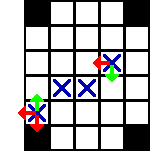
\includegraphics[width=\textwidth]{imgs/verifDepl}
			\end{block}
		\end{column}
		\begin{column}{0.49\textwidth}
			Vérifications :
			\begin{itemize}
				\item
					Déplacement dans la grille
				\item
					Déplacement sur case jouable
				\item
					Cases côtes à côtes
				\item
					Alignement de 3 ou plus
			\end{itemize}
		\end{column}
	\end{columns}
\end{frame}

\begin{frame}{Deplacement - détection et destruction}
	\begin{columns}
		\begin{column}{0.49\textwidth}
			\begin{block}{Détection}
				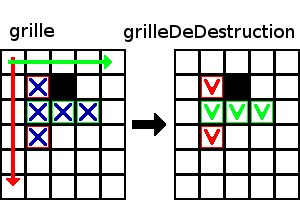
\includegraphics[width=\textwidth]{imgs/Detection}
			\end{block}
		\end{column}
		\begin{column}{0.49\textwidth}
			\begin{block}{Destruction}
				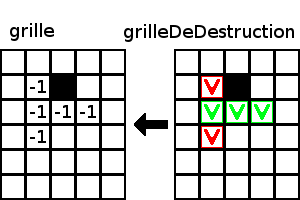
\includegraphics[width=\textwidth]{imgs/Destruction}
			\end{block}
		\end{column}
	\end{columns}
\end{frame}

\begin{frame}{Deplacement - remplacement}
	\begin{columns}
		\begin{column}{0.49\textwidth}
			\begin{block}{Tri des -1}
				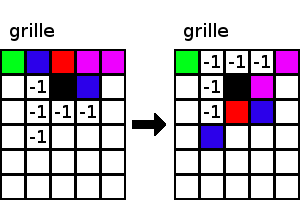
\includegraphics[width=\textwidth]{imgs/Remplacement1}
			\end{block}
		\end{column}
		\begin{column}{0.49\textwidth}
			\begin{block}{Tirage aléatoire des cases}
				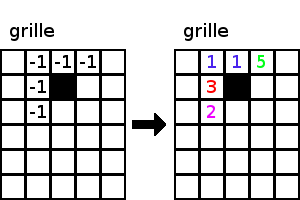
\includegraphics[width=\textwidth]{imgs/Remplacement2}
			\end{block}
		\end{column}
	\end{columns}
\end{frame}
